%%%%%%%%%%%%%%%%%%%%%%%%%%%%%%%%%%%%%%%%%
% Beamer Presentation
% LaTeX Template
% Version 1.0 (10/11/12)
%
% This template has been downloaded from:
% http://www.LaTeXTemplates.com
%
% License:
% CC BY-NC-SA 3.0 (http://creativecommons.org/licenses/by-nc-sa/3.0/)
%
%%%%%%%%%%%%%%%%%%%%%%%%%%%%%%%%%%%%%%%%%

%----------------------------------------------------------------------------------------
%	PACKAGES AND THEMES
%----------------------------------------------------------------------------------------

\documentclass{beamer}

\mode<presentation> {

% The Beamer class comes with a number of default slide themes
% which change the colors and layouts of slides. Below this is a list
% of all the themes, uncomment each in turn to see what they look like.

%\usetheme{default}
%\usetheme{AnnArbor}
%\usetheme{Antibes}
%\usetheme{Bergen}
%\usetheme{Berkeley}
%\usetheme{Berlin}
%\usetheme{Boadilla}
%\usetheme{CambridgeUS}
%\usetheme{Copenhagen}
%\usetheme{Darmstadt}
%\usetheme{Dresden}
%\usetheme{Frankfurt}
%\usetheme{Goettingen}
%\usetheme{Hannover}
%\usetheme{Ilmenau}
%\usetheme{JuanLesPins}
%\usetheme{Luebeck}
\usetheme{Madrid}
%\usetheme{Malmoe}
%\usetheme{Marburg}
%\usetheme{Montpellier}
%\usetheme{PaloAlto}
%\usetheme{Pittsburgh}
%\usetheme{Rochester}
%\usetheme{Singapore}
%\usetheme{Szeged}
%\usetheme{Warsaw}

% As well as themes, the Beamer class has a number of color themes
% for any slide theme. Uncomment each of these in turn to see how it
% changes the colors of your current slide theme.

%\usecolortheme{albatross}
%\usecolortheme{beaver}
%\usecolortheme{beetle}
%\usecolortheme{crane}
%\usecolortheme{dolphin}
%\usecolortheme{dove}
%\usecolortheme{fly}
%\usecolortheme{lily}
%\usecolortheme{orchid}
%\usecolortheme{rose}
%\usecolortheme{seagull}
%\usecolortheme{seahorse}
%\usecolortheme{whale}
%\usecolortheme{wolverine}

%\setbeamertemplate{footline} % To remove the footer line in all slides uncomment this line
%\setbeamertemplate{footline}[page number] % To replace the footer line in all slides with a simple slide count uncomment this line

%\setbeamertemplate{navigation symbols}{} % To remove the navigation symbols from the bottom of all slides uncomment this line
}

\usepackage{graphicx} % Allows including images
\usepackage{booktabs} % Allows the use of \toprule, \midrule and \bottomrule in tables

%----------------------------------------------------------------------------------------
%	TITLE PAGE
%----------------------------------------------------------------------------------------

\title[Prandtl Investigation]{The Prandtl Lift Distribution Investigation} % The short title appears at the bottom of every slide, the full title is only on the title page

\author{Niel Agenbag} % Your name
\institute[Unaffiliated] % Your institution as it will appear on the bottom of every slide, may be shorthand to save space
{
Unaffiliated \\ % Your institution for the title page
\medskip
\textit{Ludwigprandtlwing@gmail.com} % Your email address
}
\date{\today} % Date, can be changed to a custom date

\begin{document}

\begin{frame}
\titlepage % Print the title page as the first slide
\end{frame}

\begin{frame}
\frametitle{Overview} % Table of contents slide, comment this block out to remove it
\tableofcontents % Throughout your presentation, if you choose to use \section{} and \subsection{} commands, these will automatically be printed on this slide as an overview of your presentation
\end{frame}

%----------------------------------------------------------------------------------------
%	PRESENTATION SLIDES
%----------------------------------------------------------------------------------------

\section{Introduction and Goals}

\begin{frame}
\frametitle{Introduction}
\begin{itemize}
\item An alternative to the elliptical lift distribution exists from Prandtl's work in 1933 \cite{Prandtl1933} and should be investigated 
\item The Prandtl lift distribution could potentially lead to 11\% less induced drag for the same amount of structure compared to the elliptical lift distribution
\item It has applications in tailless aircraft design and should be investigated
\item Aircraft development is time consuming and expensive and way has to be found to make possible investigation of the Prandtl lift distribution
\end{itemize}
\end{frame}

\begin{frame}
\frametitle{Introduction}
\begin{itemize}
\item This presentation will suggest an open source hardware and analysis framework for such an investigation 
\item Firstly the Prandtl lift distribution will be discussed
\item Existing work will be presented
\item The work on a small glider will be presented
\item Steps for future work will be suggested
\end{itemize}
\end{frame}


\begin{frame}
\frametitle{Disclaimer}

\begin{itemize}
\item The author is not an aerodynamicist - if there are errors it needs to be treated with understanding.
\item This is investigation a hobby project of the author and associates - it is not a full time occupation.  
\item The investigation seeks to answer questions such as `How can engineering be done in new ways' and `How can aircraft be more efficient'
\item As such the investigation is not an end in itself.
\end{itemize}

\end{frame}


\begin{frame}
\frametitle{Disclaimer}

We do not pretend to know the answer.

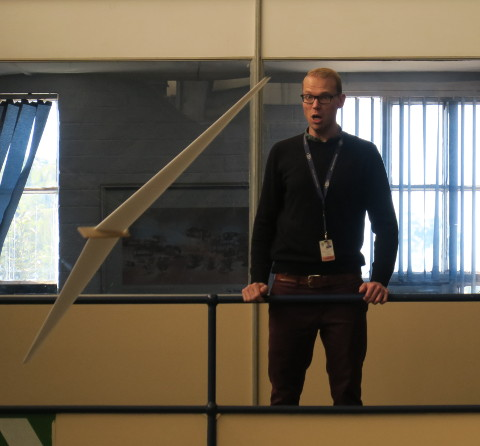
\includegraphics[width = 0.5\textwidth]{Pictures/NoIdea.JPG}

\end{frame}


\section{Prandtl's 1933 lift distribution}

\begin{frame}
\frametitle{The Prandtl lift distribution}
\begin{itemize}
\item Developed following the elliptical lift distribution
\item Leads to 11\% less induced drag for 22\% more span, but the same root bending moment
\end{itemize}


Show graph of the elliptical and Prandtl on the same picture.

Show the non-constant downwash and the upwash at the tips.

Quick rundown of theory from the NASA paper


List all the potential gains from this distribution (Less area parasitic, no yaw control necessary because no adverse yaw, leading to less drag, better handling qualities for tailless aircraft)

Show the equation of the CL local from the patent.

Talk about the negatives:  Must still prove all these claims and this will cost money.
Nickel and Wohlfahrt specifically devote a paragraph stating that this lift distribution is not worth it.  These are risks.
Larger span means that it would find limited application in commercial aviation due to existing infrastructure.


\end{frame}


\section{Existing work}


\begin{frame}
\frametitle{Existing work}
\begin{itemize}
\item NASA project initiated by Al Bowers
\item See more about it at https://www.nasa.gov/centers/armstrong/news/FactSheets/FS-106-AFRC.html
\item A technical paper (“On Wings of the Minimum Induced Drag: Spanload Implications for Aircraft and Birds,” NASA/TP – 2016-219072) on the research has been published
https://ntrs.nasa.gov/archive/nasa/casi.ntrs.nasa.gov/20160003578.pdf
\item A patent was obtained to prevent exclusive use by individuals or companies of the concept
\end{itemize}
\end{frame}


\begin{frame}
\frametitle{Existing work}

The Prandtl D aircraft

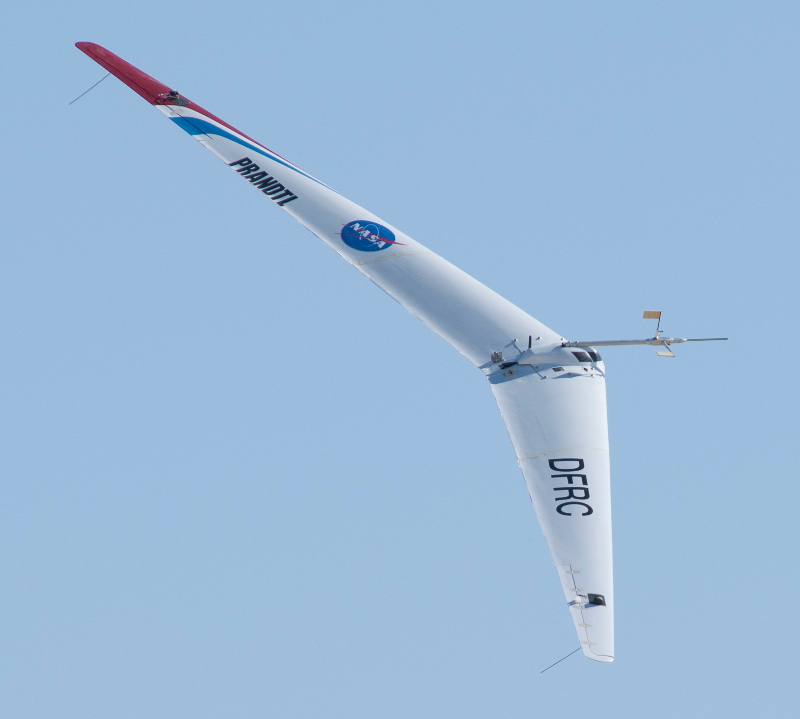
\includegraphics[width = 0.8\textwidth]{Pictures/PrandtlDflight.jpg}


\end{frame}


\begin{frame}
\frametitle{Existing work}
\begin{itemize}
\item The Prandtl D has proven that the Prandtl lift distribution has proverse yaw.
\end{itemize}
\end{frame}


\section{The Prandtl Investigation}

\begin{frame}
\frametitle{The Prandtl Investigation}

\begin{itemize}
\item The Prandtl investigation is an independent fork of a NASA Prandtl wing project.
\item The investigation will use a tailless aircraft concept to investigate the Prandtl lift distribution.  This aircraft is a research vehicle intended to investigate the bell shaped lift distribution as suggested by Ludwig Prandtl in his 1933 paper on the efficiency of wings with a specific design mass and no span limitation.
\end{itemize}

\end{frame}


\begin{frame}
\frametitle{The Prandtl Investigation}

The goals of the project are somewhat different from the NASA paper.  

\begin{itemize}
\item The paper focussed on proving the existence of proverse yaw with the Prandtl lift distribution as well as 
\item postulating that birds most likely utilize the Prandtl circulation distribution as opposed to the elliptical circulation distribution.  
\end{itemize}

\end{frame}



\begin{frame}
\frametitle{The Prandtl Investigation Goals}

The goals are:

\begin{itemize}
\item Investigate whether or not a tailless aircraft designed to have a Prandtl lift distribution will have satisfactory unaugmented (no control system except for the pilot and direct gearing of the control surfaces) handling qualities.
\item Determine the performance characteristics of such an aircraft.  In particular is important to show very favourable L/D characteristics (L/D $\geq$ 53 for full scale aircraft) and laminar flow on the wing surfaces, even with reflexed profiles that are common on tailless designs.
\end{itemize}

\end{frame}


\begin{frame}
\frametitle{The Prandtl Investigation Goals}

A secondary goal of the project is:

\begin{itemize}
\item To investigate the feasibility of open hardware design using open source tools (as far as possible).  
\item To investigate whether a community of individuals can be leveraged to bootstrap innovation
\end{itemize}

\end{frame}


\begin{frame}
\frametitle{The Prandtl Investigation Goals}

\begin{itemize}
\item Use tools such as Git for product lifecycle management and to manage design projects using mainly text files as the source documents of the design.
\item Test collaboration online with known as well as anonymous collaborators in order to bootstrap mechanical/aeronautical engineering projects.
\end{itemize}

\end{frame}


\begin{frame}
\frametitle{The Prandtl Investigation Goals}

It is hoped that this project will encourage other builders to manufacture similar designs and publish their designs, software and data in a similar manner, so as to advance the state of the art of tailless aircraft in particular and engineering in general.



\end{frame}



\section{Prandtl glider built}


\subsection{Specifications}

\begin{frame}
\frametitle{Prandtl Glider Specifications}

\begin{itemize}
\item Mass = 59 grams
\item CNC polystyrene wing with twist distribution in \cite{PrandtlBowers}
\item Balsa fuselage with prestik ballast
\end{itemize}

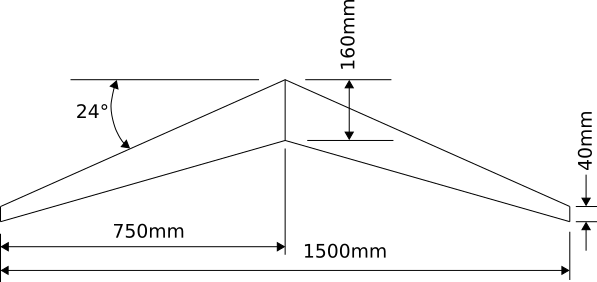
\includegraphics[width = 0.8\textwidth]{Pictures/P1Planform.png}

\end{frame}


\begin{frame}
\frametitle{Prandtl Glider Manufacturing}

Picture of the CNC of the aircraft

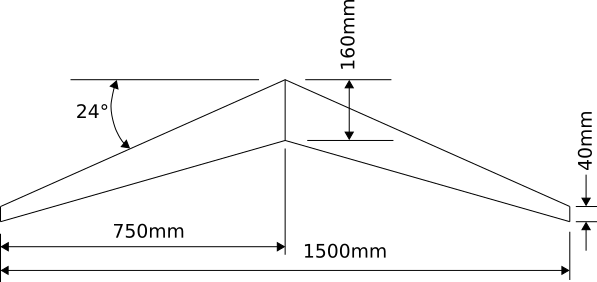
\includegraphics[width = 0.8\textwidth]{Pictures/P1Planform.png}

\end{frame}


\begin{frame}
\frametitle{Prandtl Glider Manufacturing}

Picture of the completed aircraft

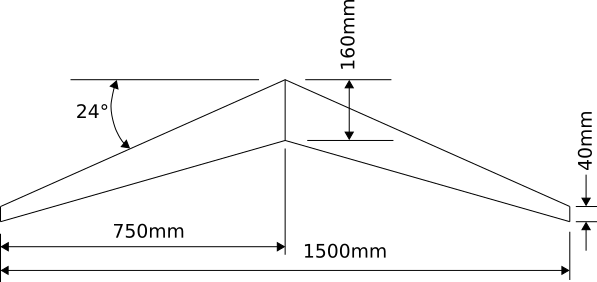
\includegraphics[width = 0.8\textwidth]{Pictures/P1Planform.png}

\end{frame}





\subsection{Calculations} % A subsection can be created just before a set of slides with a common theme to further break down your presentation into chunks

\begin{frame}
\frametitle{Neutral point calculation}
Show the neutral point calculation and show the comparison to the measured value later


\end{frame}


\begin{frame}
\frametitle{Neutral point calculation}
Show the equtions for the sink polar but specifically the drag calculation.  Show the Prandtl factor instead of the Oswald factor.  It is a measure of how close it follows the Prandtl CL local shape.
Show the value of CD obtained.


\end{frame}




\subsection{Flight tests}




\begin{frame}
\frametitle{Neutral point measurement}

\begin{itemize}
\item The advantage with model flight is that the neutral point can be iteratively determined with no safety impact.
\item Since the flights are done in the linear region, it should be reasonably representative for a full scale aircraft as well.
\end{itemize}

\end{frame}



\begin{frame}
\frametitle{Aeroelasticity}

Very large deflections possible if structure not stiff.  Note the unloaded tips.

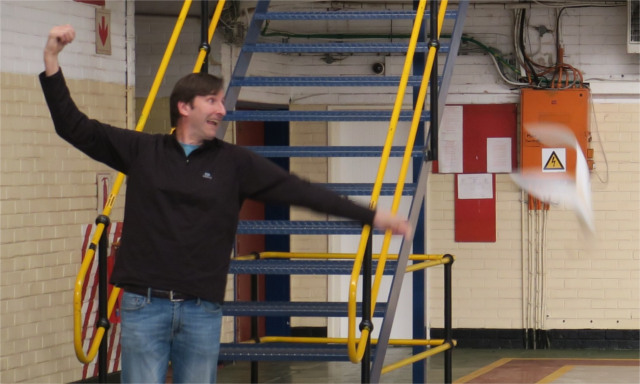
\includegraphics[width = 0.8\textwidth]{Pictures/MassiveDeflect.JPG}

\end{frame}

\subsection{Conclusions from glider}

\begin{frame}
\frametitle{Conclusions from glider}

\begin{itemize}
\item The aircraft was stable
\item Observations indicate that proverse yaw might have been achieved
\item Glide performance was poor, but is attributed to incorrect trim speed and rough finish of polystyrene wing
\item The CNC manufacturing concept was proven
\item The glider results are sufficient encouraging to continue investigation
\end{itemize}

\end{frame}





\section{Future work}


\begin{frame}
\frametitle{Suggested staged approach}

\begin{itemize}
\item Firstly a small model (1.5metre wing span, polystyrene) will be built to establish manufacturing techniques.  This step has been completed.
\item Secondly a larger 2.25m span model from balsa wood will be manufactured with better performance characteristics.  This is the current step.
\item Lastly larger prototypes have to be designed and built in order to investigate the full scale properties of this type of aircraft.  An intermediate step to the large prototype would be a 27kg all up mass aircraft.  This represents the maximum mass for a legal radio controlled aircraft in South Africa.
\item A full scale aircraft should have a 12 to 15m wing span.  
\end{itemize}

\end{frame}


\begin{frame}
\frametitle{Important notes}

\begin{itemize}
\item It is imperative that a full scale aircraft 
be manufactured since subscale tailless aircraft nearly always have satisfactory handling qualities.  Full scale tailless aircraft 
have to be built in order to investigate the vulnerabilities of tailless aircraft to gusty conditions.
\item Note the high angle of attack difference from \cite{ModelFlightNASA}
\end{itemize}

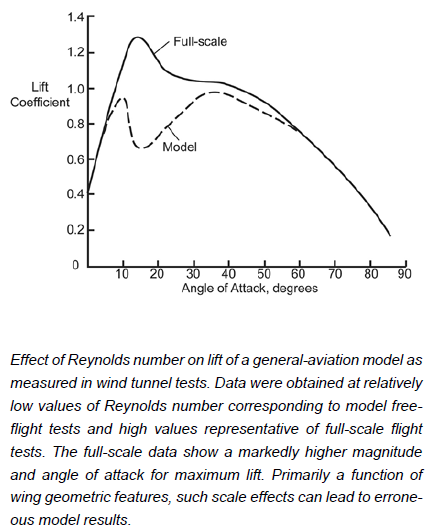
\includegraphics[width = 0.5\textwidth]{Pictures/ModelAeroVSFullSize.png}

\end{frame}




\begin{frame}
\frametitle{Important notes}

\begin{itemize}
\item The Prandtl wing aircraft is envisaged to be a remotely piloted vehicle in all stages.  This is a risk reduction strategy since the technology of tailless aircraft has inherent risks as evidenced by the literature on the subject.  Even though this is an open hardware project, it is in no way encouraged that a piloted version of this aircraft be built.
\end{itemize}

\end{frame}


\begin{frame}
\frametitle{Prandtl Evolution}

\includegraphics[width = 0.5\textwidth]{Pictures/PrandtlEvolution/PrandtlEvolution.pdf}

\end{frame}


\begin{frame}
\frametitle{Project information}

The Prandtl investigation is an open hardware, open software project.  Information about the project can be found on:  

\begin{itemize}
\item Youtube (search for ``Prandtl Aircraftwing'' on google) or paste in your browser:
https://www.youtube.com/channel/UC6F9yife2uQ-U4vDy8oB4gA
\item Instagram (ludwigprandtlwing)
\item Mail the project at: Ludwigprandtlwing@gmail.com 
\item Github (ludwigprandtlwing) https://github.com/ludwigprandtlwing
\end{itemize}

\end{frame}




\begin{frame}
\frametitle{Project information}

The Prandtl investigation is an open hardware, open software project.  As such:  

\begin{itemize}
\item You are encouraged to use all the information for your own project
\item The information should be shared as widely as possible with whomever is interested
\item You are invited to participate with us if you are interested
\item If you are so inclined, share your own work on this topic with us and all others
\end{itemize}

\end{frame}


%------------------------------------------------

\begin{frame}
\frametitle{References}
\footnotesize{
\begin{thebibliography}{99} % Beamer does not support BibTeX so references must be inserted manually as below

\bibitem{PrandtlBowers} Albion H. Bowers, and Oscar J. Murillo (2016) On Wings of the Minimum Induced Drag:  Spanload Implications for Aircraft and Birds, NASA/TP-2016-219072
\bibitem{PrandtlPatent} US Patent 9,382,000 B1, July 5, 2016, Bowers et al.
\bibitem{omegataupodcastPrandtl} Markus Voelter (2017) omega tau podcast number 256 – Flight Research at NASA Armstrong, Part 1: Subscale, http://omegataupodcast.net/256-flight-research-at-nasa-armstrong-part-1-subscale/
\bibitem{Prandtl1921} Prandtl, L.  (1921)  Applications  of  modern hydrodynamics  to  aeronautics,  NACA  Report  No  116 (Washington, DC).
\bibitem{Prandtl1933} Prandtl L (1933) Über tragfl\"ugel kleinsten induzierten widerstandes. Zeitschrift für Flugtecknik und Motorluftschiffahrt, 1 VI 1933 (M\"unchen, Deustchland).
\bibitem{ModelFlightNASA} Joseph R. Chambers, Modelling Flight - The role of dynamically scaled free-flight models in support of NASA's aerospace programs, ISBN 978-0-16-084633-5.


\end{thebibliography}
}
\end{frame}

%------------------------------------------------

\begin{frame}
\Huge{\centerline{The End}}
\end{frame}

%----------------------------------------------------------------------------------------

\end{document} 